% The satex architecture, as one picture.  Compile with pdflatex.
\documentclass[border=12pt]{standalone}

\usepackage{tikz}
\usepackage{fontawesome}
\usetikzlibrary{arrows.meta,shadows,shapes.geometric,shapes.symbols,positioning,fit,backgrounds,calc}

\pgfdeclarelayer{background}
\pgfdeclarelayer{very-background}
\pgfsetlayers{very-background,background,main}

\definecolor{BaseGray}{RGB}{66,66,66}
\colorlet{SoftGray}{BaseGray!60}
\colorlet{BackGray}{BaseGray!4}
\definecolor{TeXBlue}{RGB}{38,90,150}
\definecolor{FactGreen}{RGB}{52,120,78}
\definecolor{CacheAmber}{RGB}{176,124,26}

\begin{document}
\begin{tikzpicture}[
  Soft/.style={line join=round,line cap=round},
  font=\sffamily\small,
  node distance=9mm and 12mm,
  Stage/.style={
    fill=white,draw=BaseGray,drop shadow={fill=lightgray!50},
    signal,signal from=west,signal to=east,
    minimum width=27mm,minimum height=13mm,rounded corners=2pt,align=center},
  Hub/.style={
    fill=white,draw=BaseGray,drop shadow={fill=lightgray!50},
    rounded corners=3pt,minimum width=34mm,minimum height=12mm,align=center},
  Part/.style={
    draw=SoftGray,fill=white,rounded corners=3pt,
    minimum width=23mm,minimum height=7mm,align=center,font=\sffamily\scriptsize},
  Store/.style={
    cylinder,shape border rotate=90,aspect=0.18,draw=CacheAmber,
    fill=CacheAmber!8,minimum width=20mm,minimum height=11mm,
    align=center,font=\sffamily\scriptsize},
  Source/.style={
    draw=TeXBlue,fill=TeXBlue!6,rounded corners=3pt,
    minimum width=27mm,minimum height=8mm,align=center,font=\sffamily\scriptsize},
  Result/.style={
    draw=FactGreen,fill=FactGreen!6,rounded corners=3pt,
    minimum width=25mm,minimum height=8mm,align=center,font=\sffamily\scriptsize},
  Link/.style={draw=BaseGray,Soft,rounded corners=2.5pt,-{Kite[length=4pt,width=3pt]},thick},
  Thin/.style={draw=SoftGray,Soft,rounded corners=2.5pt,-{Kite[length=3pt,width=2.5pt]},dashed},
  Group/.style={draw=SoftGray,fill=BackGray,rounded corners=6pt,inner sep=4mm},
  Caption/.style={font=\sffamily\scriptsize\itshape,text=SoftGray},
]

% ─ inputs ────────────────────────────────────────────────────────────────────
\node[Source] (doc)   {\faFileTextO~ \texttt{paper.tex}};
\node[Source,below=5mm of doc] (proj) {\faCogs~ \texttt{latexmkrc}, \texttt{Makefile}};
\node[Source,below=5mm of proj] (cfg) {\faSliders~ \texttt{satex.yaml}};
\node[Source,below=5mm of cfg] (tree) {\faDatabase~ TEXMF trees};

\begin{pgfonlayer}{background}
  \node[Group,fit=(doc)(proj)(cfg)(tree),label={[Caption]above:input}] (inputs) {};
\end{pgfonlayer}

% ─ the pipeline ──────────────────────────────────────────────────────────────
\node[Stage,right=14mm of inputs.east,yshift=17mm] (discovery)
  {discovery\\[-1pt]{\scriptsize provider $\cdot$ platform}};
\node[Stage,below=of discovery] (format) {format\\[-1pt]{\scriptsize \texttt{latex.ltx}}};
\node[Stage,below=of format] (interp) {interpreter};
\node[Stage,below=of interp] (facts) {facts\\[-1pt]{\scriptsize what was observed}};

\node[Store,right=10mm of discovery] (index) {file index\\\textit{cached}};
\node[Store,right=10mm of format] (fcache) {format\\\textit{cached}};

% the engine, expanded
\node[Part,right=20mm of interp.east,yshift=8mm] (mouth) {mouth\\{\tiny lines $\to$ tokens}};
\node[Part,below=3mm of mouth] (gullet) {gullet\\{\tiny expansion}};
\node[Part,below=3mm of gullet] (stomach) {stomach\\{\tiny execution}};
\node[Part,right=7mm of gullet,minimum width=26mm] (state)
  {category codes\\save stack $\cdot$ meanings\\{\tiny groups, conditionals}};

\begin{pgfonlayer}{background}
  \node[Group,fit=(mouth)(gullet)(stomach)(state),
        label={[Caption]above:one token at a time}] (engine) {};
\end{pgfonlayer}

% ─ what comes out ────────────────────────────────────────────────────────────
\node[Result,right=16mm of engine.east,yshift=14mm] (defs)  {definitions $\cdot$ expansions};
\node[Result,below=4mm of defs] (loads) {loads $\cdot$ occurrences};
\node[Result,below=4mm of loads] (diag) {diagnostics};
\node[Result,below=4mm of diag,draw=BaseGray,fill=BaseGray!5] (graph)
  {dependency graph\\{\tiny \texttt{reads} $\cdot$ \texttt{defined-by} $\cdot$ \texttt{expands}}};

\begin{pgfonlayer}{background}
  \node[Group,fit=(defs)(loads)(diag)(graph),label={[Caption]above:what the run observed}] (obs) {};
\end{pgfonlayer}

% ─ analyses and output ───────────────────────────────────────────────────────
\node[Hub,below=20mm of obs.south,anchor=north] (analyses)
  {analyses\\[-1pt]{\scriptsize over the facts and the graph}};
\node[Part,left=10mm of analyses,minimum width=26mm] (lint) {lint $\cdot$ optimize};
\node[Part,below=3mm of lint,minimum width=26mm] (slice) {slice $\cdot$ controls};
\node[Part,right=10mm of analyses,minimum width=26mm] (scope) {scope $\cdot$ explain};
\node[Part,below=3mm of scope,minimum width=26mm] (query) {query $\cdot$ summary};

\node[Source,below=8mm of analyses,draw=BaseGray,fill=BaseGray!5,minimum width=46mm] (out)
  {text $\cdot$ JSON $\cdot$ SARIF $\cdot$ GitHub $\cdot$ DOT};

% ─ legend ───────────────────────────────────────────────────────────────────
\node[anchor=north west,inner sep=0pt] (legendanchor)
  at ($(facts.south west)+(-4mm,-26mm)$) {};
\node[Part,right=0mm of legendanchor,minimum width=15mm,
      draw=TeXBlue,fill=TeXBlue!6] (lgin) {input};
\node[Store,right=4mm of lgin,minimum width=14mm,minimum height=8mm] (lgcache) {cache};
\node[Part,right=4mm of lgcache,minimum width=15mm,
      draw=FactGreen,fill=FactGreen!6] (lgfact) {fact};
\node[Part,right=4mm of lgfact,minimum width=15mm,signal,signal from=west,
      signal to=east,draw=BaseGray] (lgstage) {stage};
\begin{pgfonlayer}{background}
  \node[Group,fit=(lgin)(lgcache)(lgfact)(lgstage),inner sep=3mm,
        label={[Caption]above:legend}] (legend) {};
\end{pgfonlayer}

% ─ links ─────────────────────────────────────────────────────────────────────
\draw[Link] (inputs.east) -- ++(6mm,0) |- (discovery.west);
\draw[Link] (discovery.east) -- (index.west);
\draw[Link] (index.south) -- ++(0,-4mm) -| (format.north);
\draw[Link] (format.east) -- (fcache.west);
\draw[Link] (fcache.south) -- ++(0,-5mm) -| (interp.north);
\draw[Link] (interp.east) -- (engine.west);
\draw[Link] (interp.south) -- (facts.north);
\draw[Link] (facts.east) -- ++(8mm,0) |- (obs.west);
\draw[Link] (engine.east) -- (obs.west);
\draw[Link] (obs.south) -- (analyses.north);
\draw[Link] (analyses.south) -- (out.north);
\draw[Thin] (lint.east) -- (analyses.west);
\draw[Thin] (slice.east) -- (analyses.west);
\draw[Thin] (scope.west) -- (analyses.east);
\draw[Thin] (query.west) -- (analyses.east);
% `\input` hands a new file back to the mouth.
\draw[Thin] (stomach.west) -- ++(-4mm,0) |- (mouth.west)
  node[Caption,pos=0.5,left,xshift=-1mm]{\texttt{\textbackslash input}};

\end{tikzpicture}
\end{document}
